\section{Security}

This hybrid solution allows us to use the parent chain as a reliable protector
against most of the attacks that target the PoS systems\cite{pos_attacks}. In
this section, we assume that the parent chain is well secured, and every user
has stable access to it.

\subsection{Nothing at stake}

This type of attack splits into two cases: micro forks and generational forks.

\subsubsection{Micro forks}

A malicious leader may produce blocks without any cost. They are free to create
conflicting branches within a single generation. This case is very similar to
BitcoinNG's\cite{bcng}. However, this kind of forking is not dangerous in
hyperchains. It may introduce some mess initially but becomes resolved instantly
with the next key block.

\begin{figure}[h]
	\caption{Micro fork}
	\centering
	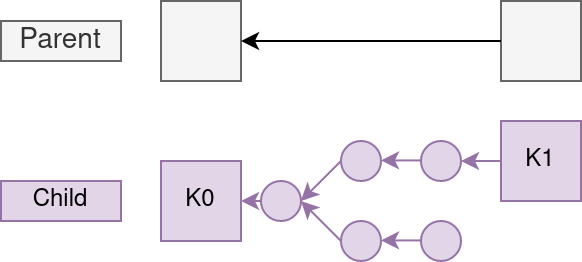
\includegraphics[scale=0.35]{microfork}
\end{figure}

\subsubsection{Generational forks}

This happens when there are multiple key blocks produced by a leader, most
likely as a consequence of a micro fork described above.

\begin{figure}[h]
	\caption{Generational Fork}
	\centering
	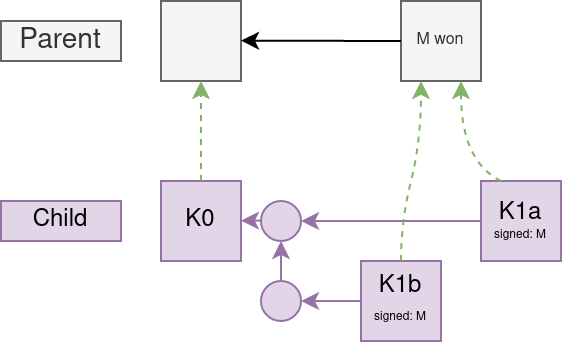
\includegraphics[scale=0.35]{genfork}
\end{figure}

The $K1a$, $K1b$, etc. are key blocks on the child chain emitted by a malicious
leader over different micro blocks. This effectively splits the network, as it
becomes unclear to which of the forks the delegates should commit.

Similarly to PoW chains, this should be solved by the rest of the network.
Eventually some peers should decide on one of the forks, breaking the balance in
the weight function proposed below. After that happens the ``heavier'' chain
shall be deemed the right one. To enforce making a decision, for every candidate
only a single commitment can be counted (most reasonably, the last one in the
parent's block).

A weight function should reflect the total staking power of those who committed
to a fork. The exact logic shall be defined in a smart contract. A simple
example would be the sum of all stakes that were backed by a commitment.

\subsection{Lazy leader}

A leader who does not produce a key block is called ``lazy''. In a case of a
lazy leader, anyone can produce a key block on behalf of them. Subsequently, the
network is most likely split in the same way as in a generational fork.
Therefore, such a situation shall be resolved the same way. This also means it
makes sense to produce key blocks even while not being a leader.

In a case in which a lazy leader submits a delayed key block, it is up to the
network whether to consider it. One may argue that a syncing peer would not have
a proof that the leader was ignored due to their laziness, but it is not
different from blacklisting. This behavior is available in almost every PoW and
PoS blockchain and in general does not cause threat, therefore we do not
consider it an issue as well.

\subsection{Stake grinding}

Since the RNG depends exclusively on the key block hash on a PoW chain, it is
impossible to predict its outcomes. One could try to mine the parent chain in a
special way, but it would require so much computational power that in most cases
it would be easier to take control by a 51\% attack.

\subsection{Long range attack}

While it is still possible to perform a long range attack, it would be
impossible to do it secretly and without preparation since the very beginning.
The commitments guarantee that the information of delegates is stored on an
immutable chain, and one would need to announce their will of mining suspicious
blocks during the entire period of the attack. This would quickly expose the
intention of the attacker and let the others prepare for a possible upcoming
attack (by blacklisting them, for example).

\subsection{Overloading parent chain}

Healthy commitment mechanism is key for fair election on a hyperchain. If some
of the delegates get prevented from publishing commitment transactions on the
parent their chances of becoming a leader will vanish regardless of their stake.
This is a vulnerable point of the system. On most blockchains there is a
limitation on the number/total size of transactions in a single block. A
malicious leader could send numerous commitments to fill the entire block
leaving no place for the others.

This strategy hands the staking value to parent's tokens in some sense. The
difference is that in this case the financial effort made to boost one's chances
of being elected is disposable (as long as the attacker did not mine that
block---but then they could just reject other commitments). At the time of
writing the costs of performing such an attack are huge on most blockchains, and
it is almost impossible to sustain it for a longer time. Note that in order to
take full control over just a single generation the attacker would need to
invest funds equal to significantly extended transaction fee multiplied by the
network throughput hoping that every other commitment will get superseded by
\textit{every} of their spam transaction. If it is not enough, performing an
election every $k_{> 1}$th block would greatly amplify the required effort.

\subsection{No commitments}

It may be the case that no one commitments to a key block, or that a miner on
the parent chain does not include any commitment. We propose that the smart
contract responsible for handling elections should decide on what happens in
that case. For example, a ``lazy leader'' scenario may be utilized; the
previous leader may take over; or the election may be reevaluated with the
candidates from the previous generation.
